\documentclass{svproc}
\usepackage{graphicx}
\usepackage{amsmath,amssymb,amsfonts}
\usepackage{booktabs}
\usepackage{url}
\usepackage{tikz}
\usetikzlibrary{positioning,arrows.meta}
\def\UrlFont{\rmfamily}

\begin{document}
\mainmatter
\title{Steering a Network with Its Own Reflection: True, False, and Noise Self-Model Broadcasts in an Evolving Multi-Agent Network}
\titlerunning{Steering a Network with Its Own Reflection}
\author{Ivan Bhargava}
\authorrunning{I. Bhargava}
\institute{Independent Researcher\\
\email{ivan.bhargava@example.com}\\ WWW home page:
\texttt{https://github.com/Ivan825/Project-ONE}}

\maketitle

\begin{abstract}
Many networks respond to measurements of their own state: markets to indices, organizations to metrics, platforms to trending signals. We present a controlled laboratory for this reflexive loop: an evolving agent population forms an adaptive network whose macrostate is compressed into a self-model and broadcast back --- accurately, distorted, or as matched-bandwidth noise. Across 927 deterministic runs with paired seeds and pre-specified outcomes: measurement without broadcast is causally inert; under corrective responses false self-models pull the macrostate toward themselves far more strongly than matched noise (paired rank-biserial $r=0.84$--$0.88$), and realistically structured descriptions steer strongest --- a replayed genuine self-model from another run out-steers both; which lies come true depends on the response regime, an alarmist lie flipping from self-defeating under corrective responses to strongly self-fulfilling under conformist ones; and heritable attention to the broadcast declines across generations with its unreliability: populations fed false self-models evolve to ignore their observer.
\keywords{adaptive networks, agent-based modeling, reflexivity, self-fulfilling dynamics, evolution of trust, network resilience}
\end{abstract}

\section{Introduction}
Adaptive networks --- graphs whose topology coevolves with the dynamical states
of their nodes --- are a central object of network science
\cite{gross2008adaptive,holme2012temporal}. A distinctive subclass has received
far less controlled attention: networks that respond to \emph{descriptions of
themselves}. Financial markets move on published indices computed from their
own trades \cite{soros2013fallibility}; universities restructure around
rankings derived from their own behavior \cite{espeland2007rankings};
recommendation platforms amplify items \emph{because} an internal measurement
declared them trending. In each case a macroscopic measurement of the system is
compressed, published, and re-enters the system as an input to microscopic
decisions --- a loop Merton called the self-fulfilling prophecy
\cite{merton1948self} and whose measure-distorting variant is known as
Goodhart's law \cite{strathern1997improving}.

Empirical study of this loop is confounded: in real systems one can rarely
withhold the measurement, falsify it in controlled directions, or replay
history under identical randomness. We therefore built a minimal simulated
world in which the loop can be opened, closed, and corrupted at will, where
every run is exactly reproducible from a configuration and seed, and where
agents are deliberately simple --- transparent trait vectors rather than
learned policies --- so every pathway from broadcast to response is
inspectable.

Our contributions are: (1) an open, deterministic experimental platform
coupling an evolving agent ecology, an adaptive interaction network, a global
observer, and a controllable broadcast channel; (2) a six-condition causal
design that separates the effect of \emph{being measured} from the effect of
\emph{being told}, the effect of \emph{self-information} from that of
\emph{stimulation} (via a matched-bandwidth noise control), and the effect of
\emph{realistic structure} from that of self-reference (via a replayed-self-model
control); (3) evidence, robust across feedback gains and two shock severities,
that under corrective response rules false self-models steer the macrostate
toward themselves far more strongly than matched noise --- noise itself
begins to steer at high gain, and steers as strongly as an inverted lie
under conformist responses --- with the steering direction set jointly by
distortion type and response regime; and (4) we demonstrate, in an
ecological agent-based setting, that \emph{attention to a collective
self-model is itself a heritable, evolvable trait} whose population mean
declines with the self-model's unreliability.
Figure~\ref{fig:loop} summarizes the design.


\begin{figure}[t]
\centering
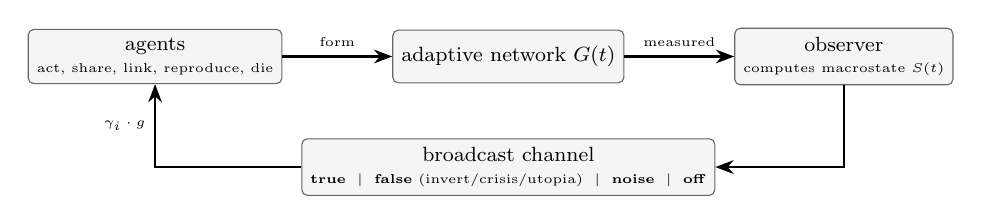
\begin{tikzpicture}[node distance=1.15cm, every node/.style={font=\footnotesize}, scale=0.93, every node/.append style={transform shape}]
\tikzstyle{box}=[rectangle, rounded corners=2pt, draw=black!60, fill=black!4, minimum height=0.72cm, minimum width=2.5cm, align=center]
\node[box] (agents) {agents\\[-1pt]{\tiny act, share, link, reproduce, die}};
\node[box, right=1.5cm of agents] (net) {adaptive network $G(t)$};
\node[box, right=1.5cm of net] (obs) {observer\\[-1pt]{\tiny computes macrostate $S(t)$}};
\node[box, below=0.75cm of net] (chan) {broadcast channel\\[-1pt]{\tiny \textbf{true} $\;\vert\;$ \textbf{false} (invert/crisis/utopia) $\;\vert\;$ \textbf{noise} $\;\vert\;$ \textbf{off}}};
\draw[-{Stealth}, thick] (agents) -- node[above]{\tiny form} (net);
\draw[-{Stealth}, thick] (net) -- node[above]{\tiny measured} (obs);
\draw[-{Stealth}, thick] (obs) |- (chan);
\draw[-{Stealth}, thick] (chan) -| node[pos=0.75, left]{\tiny $\gamma_i \cdot g$} (agents);
\end{tikzpicture}
\caption{The reflexive loop and its corruption points. Local actions generate
the network; the observer compresses it into a self-model; the broadcast
channel returns it truthfully, distorted, as noise, or not at all. Responses
are scaled by heritable sensitivity $\gamma_i$ and global gain $g$.}
\label{fig:loop}
\end{figure}

\section{Related Work}
\textbf{Adaptive and temporal networks.} Coevolution of state and topology is
surveyed in \cite{gross2008adaptive,holme2012temporal}; our model belongs to
this family, with births, deaths and rewiring driven by agent decisions.
Robustness of networks to random and targeted node removal is classical
\cite{albert2000error}; we use targeted hub removal as a standardized
perturbation rather than an object of study.
\textbf{Global coupling in physics.} Globally coupled oscillators and maps
show that a mean field fed back to units reshapes collective dynamics
\cite{kuramoto1984chemical}. Ours differs in two ways: the ``mean field'' is
a multidimensional, potentially \emph{false} description, and units are
born, die, and evolve.
\textbf{Reflexivity and reactive measurement.} Self-fulfilling prophecy
\cite{merton1948self}, reflexivity in markets \cite{soros2013fallibility}, and
the reactivity of rankings and metrics
\cite{espeland2007rankings,strathern1997improving} motivate our false-broadcast
conditions; we contribute a platform where these effects are dosable and
ablatable.
\textbf{Signaling and the evolution of trust.} In sender--receiver games,
receivers can evolve to ignore unreliable signals \cite{skyrms2010signals}.
Our distrust result is consonant with that theory but arises in an open
ecological population where the signal is \emph{self-referential} ---
a compressed description of the receiving population itself --- and where
attention to it is a continuous heritable trait under selection from an
energy economy, not a payoff matrix.
\textbf{Agent-based modeling.} Agent-based studies of collective opinion and
cooperation are a mainstay of this community
\cite{castellano2009statistical,perc2017statistical}; our methodology
follows the generative ABM tradition
\cite{epstein1996growing,bonabeau2002agent}, and the engine uses ideas from
Mesa \cite{kazil2020mesa} and NetworkX \cite{hagberg2008exploring}.
Multi-agent reinforcement learning treats global state as an
\emph{architectural} aid \cite{foerster2016learning}; we treat it as an
\emph{experimental variable} with controlled veracity. Populations of
language-model agents are now deployed with shared dashboards describing
their own collective state \cite{park2023generative}; the present rule-based
setting provides causally clean baselines for that regime.

\section{The Model}
\subsection{Agents and ecology}
Each agent $i$ carries a heritable trait vector
$\theta_i=(\mathrm{coop},\mathrm{expl},\mathrm{risk},\mathrm{soc},
\mathrm{share},\gamma_i)\in[0,1]^6$, where $\gamma_i$ is its
\emph{global sensitivity} --- how strongly broadcasts modulate its behavior.
Agents hold energy; each step they pay metabolism and choose one action ---
harvest, share (costly transfer to a neighbor), connect, prune, reproduce, or
idle --- sampled with probabilities proportional to trait- and state-dependent
propensities. The resource pool regenerates logistically, giving
density-dependent competition. Reproduction requires an energy threshold and
copies traits with Gaussian mutation ($\sigma=0.05$); energy exhaustion or age
causes death. Founding ages are staggered to avoid cohort artifacts.

\subsection{Observer and broadcast conditions}
Every $\Delta t=10$ steps the observer computes the macrostate $S(t)$:
population, fragmentation (1 minus largest-component share), degree- and
betweenness-concentration, Freeman centralization \cite{freeman1978centrality},
per-capita costly-helping rate, energy Gini, and turnover, plus mean trait
values (logged, never broadcast). The broadcast $b(t)$ carries five of these
components, each normalized to $[0,1]$: \emph{fragmentation},
\emph{centralization} (top-5\% degree share), \emph{cooperation},
\emph{inequality}, and \emph{turnover}. Six conditions define what agents
receive (Table~\ref{tab:conditions}). Distorted broadcasts come in three
modes: \emph{invert} ($b_k = 1-s_k$ componentwise), \emph{crisis} (fixed
alarming values: fragmentation $0.9$, centralization $0.9$, cooperation
$0.1$, inequality $0.9$, turnover $0.9$), and \emph{utopia} (fixed
reassuring values: $0.05$, $0.2$, $0.9$, $0.1$, $0.2$).

\subsection{Response model}
Each step, agent $i$ selects one action $a$ with probability proportional to
\begin{equation}
w_i(a,t) \;=\; w_a\big(\theta_i, x_i(t)\big) \;+\; \gamma_i\, g\, f_a\big(b(t)\big),
\label{eq:response}
\end{equation}
where $w_a(\theta_i, x_i)$ is the trait- and local-state-dependent base
propensity, $g$ is the global feedback gain, and $f_a$ is the response rule.
In the primary \emph{corrective} regime agents repair reported deficits:
$f_{\mathrm{connect}} = \max(0,\, b_{\mathrm{frag}}-0.3)$,
$f_{\mathrm{share}} = \max(0,\, 0.5-b_{\mathrm{coop}}) + 0.5\max(0,\,
b_{\mathrm{ineq}}-0.5)$,
$f_{\mathrm{harvest}} = \max(0,\, b_{\mathrm{turn}}-0.5)$, and
$f_{\mathrm{prune}} = 0.3\max(0,\, b_{\mathrm{cent}}-0.6)$.
In the \emph{conformist} regime agents imitate the reported norm instead:
$f_{\mathrm{share}} = b_{\mathrm{coop}}$,
$f_{\mathrm{prune}} = 0.5\, b_{\mathrm{frag}}$,
$f_{\mathrm{connect}} = \max(0,\, 0.6-b_{\mathrm{frag}})$, and
$f_{\mathrm{harvest}} = b_{\mathrm{ineq}}$. Two further mechanisms act on
\emph{target selection} rather than action choice, in both regimes: while
reported centralization exceeds $0.6$, a pruning agent cuts its
highest-degree neighbor (ties by id) with probability $\gamma_i$, else a
uniform neighbor; and new links attach to a neighbor-of-a-neighbor with
probability $0.7$ when available (else a uniform non-neighbor) --- an
explicit triadic-closure tendency contributing to the clustering in
Sect.~3.4. All rule constants are fixed across all experiments;
Table~\ref{tab:params} lists the model parameters.

\begin{table}[t]
\centering\footnotesize
\caption{Model parameters (defaults; campaign overrides noted in the text).}
\label{tab:params}
\begin{tabular}{@{}llll@{}}
\toprule
initial population & 150 & observer interval $\Delta t$ & 10 steps\\
population cap & 1200 & feedback gain $g$ & 0.8 (swept 0.2--1.6)\\
initial edges per agent & 3 (random) & mutation $\sigma$ & 0.05\\
initial energy & 20 & initial traits & mean 0.5, s.d. 0.15\\
resource capacity $K$ & 6000 & reproduction threshold / cost & 30 / 16\\
base regeneration & 60/step & min.\ reproduction age & 15 steps\\
regeneration rate $r$ & 0.12 & lifespan (mean $\pm$ s.d.) & $400 \pm 80$ steps\\
harvest cap & 2.5/step & action cost / share amount & 0.25 / 3.0\\
metabolism & 0.8/step & run length & 3000--4000 steps\\
shock time $t_{\mathrm{shock}}$ & 2000 & & \\
\bottomrule
\end{tabular}
\end{table}

\begin{table}[t]
\centering\footnotesize
\caption{Experimental conditions. All start from matched parameter
distributions with paired random seeds.}
\label{tab:conditions}
\setlength{\tabcolsep}{4pt}
\resizebox{\textwidth}{!}{%
\begin{tabular}{@{}llll@{}}
\toprule
Condition & Observer & Agents receive & Role\\
\midrule
A --- Local only & off & nothing & baseline\\
B --- Observed, blind & on & nothing & measurement control\\
C --- True feedback & on & accurate $S(t)$ & main treatment\\
F --- False feedback & on & distorted $S(t)$ & reflexivity probe\\
N --- Noise feedback & on & uniform random, matched ranges & stimulation control\\
R --- Replayed self-model & on & another run's genuine $S(t)$ & structure control\\
\bottomrule
\end{tabular}}
\end{table}

\subsection{Emergent network structure}
The interaction networks that emerge are dense, clustered, and heterogeneous:
at $t=2{,}000$ the giant component has short characteristic path lengths
($L\approx1.9$--$2.5$), high clustering ($1.8$--$2.4\times$ an
Erd\H{o}s--R\'enyi null of matched size and density), and a broad degree
spread (coefficient of variation $0.6$--$0.75$; maximum degree
$2$--$2.5\times$ the mean). Against the stricter degree-preserving
(configuration-model) null, however, most of the clustering excess is
accounted for by the degree sequence (observed/null ratios $1.0$--$1.6$
across seeds and conditions), so we characterize the substrate simply as a
small, dense, degree-heterogeneous network rather than claiming a
small-world regime. The point relevant to what follows is that feedback acts
on a heterogeneous, clustered graph rather than a homogeneous mixing
population.

\subsection{Reproducibility}
The simulation is deterministic given (configuration, seed): one PRNG drives
all choices, agents act in sorted order, and a state hash certifies replay;
identical hashes were verified across operating systems and machines. All
code, configurations, and analysis scripts are public.

\section{Experimental Design}
The standardized shock removes, in a single step at $t_{\mathrm{shock}}=2000$
(all campaigns), the
highest-degree living agents (ties broken by agent id): a fixed 10 hubs in
the mild variant, the top $\max(1, \lfloor 0.4\,|V_{\mathrm{live}}|\rfloor)$ in the
harsh variant. Four outcomes were fixed before the first campaign: (1)
post-shock recovery time --- the first $t > t_{\mathrm{shock}}$ at which the
living population regains $90\%$ of its pre-shock baseline, defined as its
mean over $[t_{\mathrm{shock}}{-}500,\, t_{\mathrm{shock}})$; (2) mean
post-shock fragmentation; (3) per-capita
costly-helping rate; (4) \emph{story pull}: with $s_k(t)$ the value of macrostate component
$k$ at observer tick $t$, $b_k(t)$ the broadcast value, and
$\varepsilon=0.02$,
\begin{equation}
P \;=\; \Big\langle\, \mathrm{sign}\big(b_k(t)-s_k(t)\big)\,
\big(s_k(t{+}1)-s_k(t)\big) \,\Big\rangle_{(t,k)\,:\,|b_k(t)-s_k(t)|>\varepsilon},
\label{eq:pull}
\end{equation}
averaged with equal weight over all qualifying (tick, component) pairs
across the five broadcast components; $P>0$ means the macrostate moves
toward the broadcast where the two differ, and its magnitude is bounded by
the largest per-tick component change. The threshold $\varepsilon$ makes $P$
well defined under false and noise broadcasts (and undefined for C, whose
broadcast equals the current state); results are insensitive to its value
--- for $\varepsilon\in\{0.01, 0.02, 0.05\}$ the paired F-vs-N effect is
$r = 0.88, 0.88, 0.86$ (all $p<6\times10^{-6}$) and the steering hierarchy
reported below is unchanged. Campaigns: a \emph{flagship} run (conditions
A/B/C/F$_{\mathrm{invert}}$/N $\times$ 50 paired seeds, mild shock), a
\emph{harsh-shock} replication (removal of 40\% of hubs, $\times$30 seeds), and
a \emph{sensitivity sweep} (feedback gain $g\in\{0.2,0.8,1.6\}$ $\times$
\{A, C, F$_{\mathrm{invert}}$, F$_{\mathrm{crisis}}$, F$_{\mathrm{utopia}}$,
N\} $\times$ 20 seeds), a \emph{scale check} re-running the core conditions with doubled population and resource capacity, a \emph{response-regime campaign} repeating all broadcast conditions with conformist agents (15 seeds per cell), and a \emph{replay control} (30 receiving runs paired with the harsh-shock seed list, plus 15 auxiliary source runs that generate the replayed trajectories): $250+150+360+90+32+30+15 = 927$ runs executed in total, each of 3{,}000--4{,}000 steps. Because conditions share seed lists, the design is paired; the primary
analysis is a Wilcoxon signed-rank test on per-seed differences, reported
with the matched-pairs rank-biserial correlation $r$ and a bootstrap 95\%
CI on the median difference. Unpaired Mann--Whitney $U$ with Cliff's
$\delta$ is retained as a robustness check and agrees with the paired
analysis throughout; all other logged measures are exploratory.

\section{Results}

\begin{table}[t]
\centering
\caption{Primary paired comparisons (Wilcoxon signed-rank on per-seed
differences; matched-pairs rank-biserial $r$; bootstrap 95\% CI of the median
difference). FL = flagship (50 pairs), HS = harsh shock (30 pairs).}
\label{tab:stats}
\begin{tabular}{@{}llrrr@{}}
\toprule
Outcome & Comparison & $\Delta$median [CI] & $r$ & $p$\\
\midrule
every outcome (FL, HS) & B vs A & all differences $\equiv 0$ & --- & ---\\
story pull (FL) & F vs N & $+0.0055$ $[0.0033, 0.0064]$ & $0.84$ & $1.1\times10^{-8}$\\
story pull (HS) & F vs N & $+0.0065$ $[0.0043, 0.0078]$ & $0.88$ & $3.2\times10^{-6}$\\
story pull (HS) & R vs N & $+0.0212$ $[0.0181, 0.0243]$ & $1.00$ & $1.9\times10^{-9}$\\
cooperation (FL) & C vs A & $+0.200$ $[0.172, 0.239]$ & $1.00$ & $8.9\times10^{-15}$\\
cooperation (HS) & C vs A & $+0.209$ $[0.170, 0.248]$ & $0.99$ & $9.3\times10^{-9}$\\
fragmentation (FL) & F vs A & $-0.017$ $[-0.034, -0.006]$ & $-0.53$ & $9.5\times10^{-4}$\\
$\Delta\bar\gamma$ (HS) & F vs A & $-0.336$ $[-0.456, -0.281]$ & $-1.00$ & $1.9\times10^{-9}$\\
$\Delta\bar\gamma$ (HS) & N vs A & $-0.257$ $[-0.333, -0.218]$ & $-0.98$ & $1.9\times10^{-8}$\\
recovery time (FL, HS) & C, F, N vs A & $\Delta$median $= 0$ & $|r|<0.5$ & $>0.22$\\
\bottomrule
\end{tabular}
\end{table}

Table~\ref{tab:stats} summarizes the pre-specified comparisons; the following subsections unpack them.

\subsection{Measurement alone is causally inert}
Under paired seeds, condition B is trajectory-identical to A: every per-seed
difference is exactly zero, on every outcome, in both the flagship and
harsh-shock campaigns. The
instrument acquires causal power only when it broadcasts --- a validation that
the design isolates the channel of interest.

\subsection{A false self-model pulls the macrostate toward itself}
Except where stated otherwise, all results concern the primary corrective
regime; Sect.~\ref{sec:regime} shows how they change under conformity. Story pull (Eq.~\ref{eq:pull}) under the inverted false broadcast exceeds
the noise control at every gain tested (paired: flagship $\Delta$median
$+0.0055$, $r=0.84$, $p\!\approx\!1.1\times10^{-8}$; harsh shock
$+0.0065$, $r=0.88$, $p\!\approx\!3.2\times10^{-6}$). Tested directly
against zero (harsh shock; median $P$ with bootstrap 95\% CI of the median;
one-sample Wilcoxon signed-rank), the pull is positive in every broadcast
condition: F median $0.0078$ $[0.0066, 0.0100]$; R (below) $0.0241$
$[0.0197, 0.0265]$ (both $p\!\approx\!1.9\times10^{-9}$); N $0.0021$
$[0.0009, 0.0038]$ ($p\!\approx\!10^{-3}$). Decomposed by
component, the aggregate pull is carried chiefly by the turnover
($\approx\!0.033$) and cooperation ($\approx\!0.005$) components; the
structural components are net-neutral, because the corrective over-connection
documented below cancels drift toward the reported high fragmentation.
Relative to noise the effect is strongest at \emph{low} gain (ratio
$\approx 7$ at $g=0.2$): a quiet, systematic lie out-steers loud noise,
while at high gain noise itself begins to steer (Fig.~\ref{fig:sweep},
middle). Spillovers are substantial: the inverted broadcast reduces
post-shock fragmentation relative to baseline (flagship paired
$\Delta$median $-0.017$, $r=-0.53$, $p\!\approx\!1\times10^{-3}$;
directionally consistent but not significant in the harsh-shock replication,
$p=0.28$) because agents persistently told the network is fragmenting
over-connect it (Fig.~\ref{fig:netpair}).

\paragraph{Realistic structure grades the steering channel.} A stronger
structured control replaces the broadcast with a \emph{replayed genuine
self-model}: the recorded $S(t)$ trajectory of an observed-but-blind run with
a different seed (condition R; 30 receiving runs sharing the harsh-shock seed
list, each replaying one of 15 source trajectories) --- realistic marginals
and temporal coherence, no self-reference. The resulting steering hierarchy
is R $>$ F $>$ N (medians $0.024$, $0.008$, $0.002$; paired over the 30
shared seeds, R vs N and F vs R both $|r|=1.00$,
$p\!\approx\!1.9\times10^{-9}$). The result does not depend on the reuse of
source trajectories: restricted to one receiver per source ($n=15$
independent trajectories), R exceeds F and N in every pair ($r=1.00$,
$p=6.1\times10^{-5}$ for both), and a source-clustered bootstrap over the
full sample gives mean differences R$-$F $+0.0148$ $[0.0121, 0.0173]$ and
R$-$N $+0.0207$ $[0.0178, 0.0235]$. Nor is it explained by how often
responses fire: mean discrepancy $\langle|b_k-s_k|\rangle$ is $0.64$ (F),
$0.37$ (N), and only $0.10$ (R), and F holds four of five corrective rules
active on $\geq 90\%$ of ticks against a mostly quiescent profile under R
--- R steers most while activating least. R is of course also a false
description of the receiving network --- a \emph{realistically structured}
one, true of a sibling world. Steering power is therefore graded by the
realism of the description's structure, and the channel responds to that
structure, not to persistence or stimulation volume alone.

\paragraph{Structural consequences.} Broadcasts densify and flatten the
network. Relative to A (paired, harsh shock, post-transient medians), mean
degree rises by $+1.1$ under truth ($r=0.49$) and by $+3.8$/$+4.2$ under
false/noise broadcasts ($r=0.80$/$0.79$), while Freeman centralization falls
(F vs A: $-0.026$, $r=-0.74$) and betweenness concentration falls (F:
$-0.007$, $r=-0.67$; N similar): the fed-back network becomes denser and
less hub-dominated than the silent one.

\begin{figure}[t]
\centering

\includegraphics[width=\textwidth]{sweep_summary.png}
\caption{Sensitivity sweep (40\% hub-removal shock; 20 seeds per cell;
medians). Left: evolved change in mean global sensitivity $\gamma$ ---
attention to the self-model declines in proportion to broadcast
unreliability and gain; the flattering (utopia) lie tracks the no-feedback
baseline exactly. Middle: story pull toward the broadcast. Right: cooperation
rate.}
\label{fig:sweep}
\end{figure}


\begin{figure}[t]
\centering
\includegraphics[width=0.88\textwidth]{network_pair.png}
\caption{The same world under two mirrors. Two runs from an identical seed at
$t=2000$: without feedback (left) and under the inverted false broadcast (right),
which persistently reports fragmentation and thereby drives over-connection
(mean degree $22.4$ vs $11.2$) and elevated costly helping. Node size encodes
energy; color encodes generation.}
\label{fig:netpair}
\end{figure}

\subsection{The type of lie sets the direction}
The three distortion modes produce qualitatively different regimes
(Fig.~\ref{fig:sweep}). The \emph{inverted} self-model, always reporting the
mirror of reality, generates the strongest pull: it keeps every corrective
response permanently active and thereby parasitizes the population's repair
machinery. The \emph{crisis} self-model is self-defeating for structure ---
corrections push fragmentation away from the alarmist report --- yet its
permanent cooperation-deficit signal mobilizes the highest costly-helping
rates observed ($0.36$--$0.45$). The \emph{utopia} self-model is behaviorally
inert: because responses fire only on reported deficits, a flattering
broadcast triggers nothing and is indistinguishable from disconnecting the
channel, at every gain. Under purely corrective response rules, flattery
equals silence. We note the caveat here rather than in the discussion: the
first-order \emph{directions} of these responses follow from the corrective
rules (Eq.~\ref{eq:response}) by construction and are not claimed as
discoveries; what is not built in is the magnitude asymmetry between
distortion types, the spillovers to non-targeted structure, and the
evolutionary consequences below.

\subsection{The response regime decides which lies come true}
\label{sec:regime}
Repeating all broadcast conditions with conformist agents reverses the
taxonomy exactly as the mechanism predicts (Table~\ref{tab:regime}). The
\emph{crisis} lie, self-defeating under correction, becomes strongly
self-fulfilling under conformity: told the world is fragmenting, imitators cut
ties and fragmentation rises an order of magnitude above baseline ($0.400$ vs
$0.038$). The \emph{utopia} lie flips from behaviorally inert to benevolently
self-fulfilling: ``everyone cooperates'' becomes true by imitation
(cooperation $0.428$, the highest observed in any condition). Under conformity
noise steers as strongly as the inverted lie, since imitation amplifies any
reported value. Which false self-models come true is therefore a property of
the lie--response pair, not of the lie alone.

\begin{table}[t]
\centering\footnotesize
\caption{The same lie under two response regimes (medians; harsh shock,
$g=0.8$). Baseline (A): cooperation $0.18$, fragmentation $0.038$.}
\label{tab:regime}
\begin{tabular}{@{}lllll@{}}
\toprule
Lie & \multicolumn{2}{c}{Corrective} & \multicolumn{2}{c}{Conformist}\\
 & coop. & fragm. & coop. & fragm.\\
\midrule
Invert & $0.27$ & $0.021$ & $0.42$ & $0.054$\\
Crisis & $0.36$ & $0.025$ & $0.26$ & $\mathbf{0.400}$\\
Utopia & $0.19$ (inert) & $0.037$ (inert) & $\mathbf{0.428}$ & $0.025$\\
\bottomrule
\end{tabular}
\end{table}

\subsection{Populations fed lies evolve to stop listening}
Mean heritable global sensitivity $\bar\gamma$ changes over $\sim$40
generations as an emergent, unprogrammed function of broadcast quality
(Fig.~\ref{fig:trait}). At $g=0.8$ (harsh-shock campaign): no broadcast $-0.03$
(neutral drift), truth $-0.10$, noise $-0.30$ (paired $r=-0.98$), false
$-0.42$ (paired $\Delta$median $-0.336$ $[-0.456,-0.281]$, $r=-1.00$,
$p\!\approx\!1.9\times10^{-9}$). The sweep reveals a
dose--response: the decline under the false broadcast deepens from $-0.11$
($g=0.2$) to $-0.45$ ($g=1.6$) --- and at the highest gain even \emph{accurate}
feedback shows a marked decline ($-0.24$): high-impact feedback is
disfavored even when true. The utopia lie, being consequence-free, produces
no decline at all.

We state the claim at the level the data support: a systematic,
dose-dependent shift in the frequency of a heritable trait under matched
conditions, whose individual-level pathway is not a simple fecundity
gradient --- the within-run correlation between $\gamma_i$ and offspring
count is not negative under F ($\rho\approx+0.05$) --- and not
shock-mediated (F without the shock: $-0.40$ vs $-0.39$ with it; shock
victims' mean $\gamma$ exceeds the population mean by only $+0.03$). The
pathway plausibly runs through lineage survival and energy budgets
downstream of reproduction; identifying it precisely is left open.

\begin{figure}[t]
\centering

\includegraphics[width=0.55\textwidth]{fig8_trait_evolution.png}
\caption{Evolution of attention to the self-model (harsh-shock campaign,
$g=0.8$, 30 seeds per condition). Change in population-mean global
sensitivity $\bar\gamma$, run start to end. The ordering (false $<$ noise
$<$ true $<$ none) emerged from the evolutionary dynamics alone; nothing in
the rules references broadcast reliability.}
\label{fig:trait}
\end{figure}

\subsection{Accurate feedback as distributed corrective feedback}
True feedback roughly doubles costly helping (flagship: $0.397$ vs $0.179$;
paired $\Delta$median $+0.200$ $[0.172,0.239]$, $r=1.00$,
$p\!\approx\!9\times10^{-15}$; replicated under harsh shock, $r=0.99$),
rising monotonically with gain ($0.27\!\to\!0.49$); Fig.~\ref{fig:traj} shows the sustained divergence of trajectories. The loop
implements distributed corrective feedback: deficits reported at the
population level are repaired by uncoordinated individual action.


\begin{figure}[t]
\centering

\includegraphics[width=0.62\textwidth]{fig6_cooperation_traj.png}
\caption{Mean cooperation trajectories by condition (flagship campaign, 50 seeds
per condition; dashed line marks the standardized shock). Conditions A and B
coincide exactly. True and noise feedback sustain elevated cooperation; the
inverted false broadcast sustains an intermediate level.}
\label{fig:traj}
\end{figure}

\subsection{A pre-specified null result}
We detected no evidence of a feedback effect on post-shock recovery time in
any condition or campaign, even with 40\% of hubs removed (all $p>0.12$;
median $\approx 40$ steps throughout). Within the regimes tested, resilience
appears demographic --- fast regrowth --- rather than informational; we
report this pre-specified null as observed rather than adjusting the
protocol until it disappears.

\subsection{Robustness to system scale}
Re-running the core conditions (A, C, F$_{\mathrm{invert}}$, N) with doubled
initial population and proportionally scaled resources (steady-state
population $\approx 120$--$130$ vs.\ $\approx 60$) preserves every effect
under the paired analysis ($n=8$ seed pairs per condition): cooperation under
true feedback is $0.399$ vs.\ $0.188$ baseline ($\Delta$median $+0.151$
$[0.119, 0.247]$, $r=1.00$, $p=0.008$),
story pull retains F vs.\ N superiority ($\Delta$median $+0.0046$
$[0.0022, 0.0070]$, $r=0.89$, $p=0.023$), and the distrust ordering is intact
with F vs.\ A at $\Delta$median $-0.299$ $[-0.388, -0.212]$, $r=-1.00$,
$p=0.008$. The principal phenomena therefore persist under a $2\times$
increase in system scale.

\section{Discussion and Limitations}
As noted alongside the results, the first-order response directions are
encoded in the rules; the findings live one level up: the magnitude and
asymmetry of steering (graded by the realism of the description's structure;
under corrective responses consistent lies $\gg$ matched noise, strongest at
low gain), the spillovers to non-targeted structure, the regime-dependent
taxonomy of lies (exploitative / mobilizing-but-self-defeating / inert under
correction; reversed under conformity), and above all the evolutionary
layer, in which the credibility of a collective self-model becomes an
evolving property of the population. Limitations: a single ecology and
parameter family (though effects are monotone across an $8\times$ gain range
and stable under a $2\times$ scale change), fixed rule-based rather than
learned response policies, and one network per run rather than interacting
populations.

The results have a practical reading for engineered systems. Metric-driven
infrastructure --- autoscalers, observability pipelines, trending algorithms
--- constitutes exactly this loop; the false-broadcast conditions model
telemetry corruption, and the utopia result suggests that under
deficit-driven responses \emph{flattering telemetry can be operationally
equivalent to no telemetry} while raising no alarms. Documented episodes of measurement reshaping the measured system ---
from ranking reactivity in institutions \cite{espeland2007rankings} to the
degradation of Google Flu Trends once its predictions entered the environment
they forecast \cite{lazer2014parable} --- are natural empirical targets, and
connecting the model's regimes to such datasets is the clearest path to
empirical grounding. For multi-agent AI, where fleets of agents increasingly
receive dashboards of their own collective state, the evolution-of-distrust
result suggests that persistent misreporting does not merely misdirect a
population --- it degrades the control channel itself.

\section{Conclusion}
We introduced a reproducible causal laboratory for reflexive self-modeling in
adaptive networks and used it to show that (i) being measured changes nothing
while being told changes much; (ii) under corrective responses a consistent
false self-description steers a collective toward itself far more effectively
than noise --- with realistically structured descriptions steering strongest
--- while under conformist responses noise steers as strongly as an inverted
lie; (iii) which lies come true is set by the lie--response pair, not the lie
alone; and (iv) heritable attention to the collective self-model declines
across generations in proportion to the self-model's unreliability and
impact, making a population's trust in its own self-model an evolving
quantity --- one that unreliable observers spend down. Future work:
continuity under total population turnover, learned response policies, and
language-model agents.

\smallskip
\noindent\textbf{Reproducibility.} Code, configurations, all 912 stored run manifests plus the 15 replay-source trajectories, and
one-command reproduction of every figure:
\texttt{github.com/Ivan825/Project-ONE} at tag \texttt{cn2026-submission}
--- the exact state described here.


\begingroup\small
\begin{thebibliography}{19}

\bibitem{gross2008adaptive} Gross, T., Blasius, B.: Adaptive coevolutionary
networks: a review. J. R. Soc. Interface 5(20), 259--271 (2008)
\bibitem{holme2012temporal} Holme, P., Saram\"aki, J.: Temporal networks.
Phys. Rep. 519(3), 97--125 (2012)
\bibitem{soros2013fallibility} Soros, G.: Fallibility, reflexivity, and the
human uncertainty principle. J. Econ. Methodol. 20(4), 309--329 (2013)
\bibitem{espeland2007rankings} Espeland, W.N., Sauder, M.: Rankings and
reactivity: how public measures recreate social worlds. Am. J. Sociol.
113(1), 1--40 (2007)
\bibitem{merton1948self} Merton, R.K.: The self-fulfilling prophecy. Antioch
Rev. 8(2), 193--210 (1948)
\bibitem{strathern1997improving} Strathern, M.: `Improving ratings': audit in
the British university system. Eur. Rev. 5(3), 305--321 (1997)
\bibitem{albert2000error} Albert, R., Jeong, H., Barab\'asi, A.-L.: Error and
attack tolerance of complex networks. Nature 406, 378--382 (2000)
\bibitem{kuramoto1984chemical} Kuramoto, Y.: Chemical Oscillations, Waves,
and Turbulence. Springer (1984)
\bibitem{skyrms2010signals} Skyrms, B.: Signals: Evolution, Learning, and Information. Oxford Univ.\ Press (2010)
\bibitem{epstein1996growing} Epstein, J.M., Axtell, R.: Growing Artificial Societies. Brookings/MIT Press (1996)
\bibitem{bonabeau2002agent} Bonabeau, E.: Agent-based modeling: methods and
techniques for simulating human systems. PNAS 99(suppl.~3), 7280--7287 (2002)
\bibitem{kazil2020mesa} Kazil, J., Masad, D., Crooks, A.: Utilizing Python
for agent-based modeling: the Mesa framework. In: SBP-BRiMS. Springer (2020)
\bibitem{hagberg2008exploring} Hagberg, A., Schult, D., Swart, P.: Exploring
network structure, dynamics, and function using NetworkX. In: SciPy (2008)
\bibitem{foerster2016learning} Foerster, J., Assael, Y.M., de~Freitas, N.,
Whiteson, S.: Learning to communicate with deep multi-agent reinforcement
learning. In: NeurIPS (2016)
\bibitem{park2023generative} Park, J.S., O'Brien, J., Cai, C.J., Morris,
M.R., Liang, P., Bernstein, M.S.: Generative agents: interactive simulacra of
human behavior. In: UIST (2023)
\bibitem{castellano2009statistical} Castellano, C., Fortunato, S., Loreto, V.: Statistical physics of social dynamics. Rev. Mod. Phys. 81, 591--646 (2009)
\bibitem{perc2017statistical} Perc, M., Jordan, J.J., Rand, D.G., Wang, Z.,
Boccaletti, S., Szolnoki, A.: Statistical physics of human cooperation. Phys.
Rep. 687, 1--51 (2017)
\bibitem{lazer2014parable} Lazer, D., Kennedy, R., King, G., Vespignani, A.: The parable of Google Flu: traps in big data analysis. Science 343, 1203--1205 (2014)
\bibitem{freeman1978centrality} Freeman, L.C.: Centrality in social networks:
conceptual clarification. Soc. Netw. 1(3), 215--239 (1978)
\end{thebibliography}
\endgroup
\end{document}
